\documentclass[11pt,a4paper]{article}
\usepackage[margin=2.15cm]{geometry}
\usepackage[T1]{fontenc}
\usepackage[british]{babel}
\usepackage{lmodern}
\usepackage{amsmath,amssymb,amsthm}
\usepackage{booktabs,array,tabularx,longtable}
\usepackage{graphicx}
\usepackage[section]{placeins}
\usepackage[round,authoryear,sort]{natbib}
\usepackage{xurl}
\usepackage{hyperref}
\hypersetup{colorlinks=true,linkcolor=blue,citecolor=blue,urlcolor=blue,pdftitle={Majorities Without Governments: Exact Response Tensors and Constrained Coalition Formation in Sweden},pdfauthor={Mehmet Yalçın and Osman Karslı}}
\graphicspath{{figures/}}
\setlength{\parskip}{0.32em}
\setlength{\parindent}{1em}
\setlength{\tabcolsep}{5pt}
\setlength{\emergencystretch}{1.5em}
\newcolumntype{Y}{>{\raggedright\arraybackslash}X}
\renewcommand{\arraystretch}{1.12}
\newcommand{\ind}{\mathbf{1}}
\newcommand{\NR}{\mathrm{NR}}
\newcommand{\No}{\mathrm{No}}
\newcommand{\Feas}{\mathcal{F}}
\newcommand{\Reach}{\mathcal{R}}
\newcommand{\States}{\mathcal{S}}
\newtheorem{proposition}{Proposition}[section]
\providecommand{\doi}[1]{\href{https://doi.org/#1}{#1}}
\title{Majorities Without Governments:\\Exact Response Tensors and Constrained Coalition Formation in Sweden}
\author{Mehmet Yal\c{c}{\i}n\textsuperscript{*}\\[-.35em]
{\fontsize{8}{10}\selectfont\textsuperscript{*}Independent researcher, Sweden.}\\[-.35em]
{\fontsize{8}{10}\selectfont Correspondence: \href{mailto:myalcin81@gmail.com}{myalcin81@gmail.com}.}\\[-.35em]
{\fontsize{8}{10}\selectfont ORCID: \href{https://orcid.org/0009-0005-3021-8750}{0009-0005-3021-8750}.}
\and Osman Karsl{\i}\textsuperscript{\textdagger}\\[-.35em]
{\fontsize{8}{10}\selectfont\textsuperscript{\textdagger}Independent researcher.}\\[-.35em]
{\fontsize{8}{10}\selectfont E-mail: \href{mailto:theosmanuall@gmail.com}{theosmanuall@gmail.com}.}\\[-.35em]
{\fontsize{8}{10}\selectfont ORCID: \href{https://orcid.org/0009-0003-9493-3417}{0009-0003-9493-3417}.}}
\date{November 2026}
\begin{document}
\maketitle
\begin{abstract}
An electoral majority can coexist with a prolonged failure to form a government because seats, cabinet consent and parliamentary acceptance impose different requirements. We investigate the gap between arithmetic possibility and a reachable agreement using Sweden's 2026 formation episode. Official notices identify three initial exploratory assignments, a resumed assignment and two rejected prime-minister proposals; extensions of an exploratory task are not counted as failed investiture votes. We combine a finite-state model of conditional commitments with exact response tensors calculated from the complete electoral allocation and a census of 2,612 parliamentary roll calls. Six pairs of disjoint voter transfers yield 2,271 complete interior comparisons: 233 negative and 28 positive seat interactions, but 418 positive investiture-threshold interactions. In the bargaining experiment, unchanged composition conditions block agreement despite an arithmetic majority. Releasing one condition after the first, second or third formal rejection yields agreement in 37,440, 31,680 or 20,160 of 40,320 fixed proposal agendas; release after the fourth is too late. The electoral experiment produces 26 distinct seat vectors. In 15, internal concessions alone cannot restore nonrejection: external tolerance becomes necessary. Ordinary roll calls provide a separate empirical comparison: recurrent party-action agreement does not identify candidate-specific investiture commitments. Alternative party-action rules preserve the internal--external agreement boundary while identifying cost and opposition responses that depend on rule coding. The results identify exact conditional structures and observable implications for studying bargaining sequences. The accompanying repository reproduces the numerical experiments, tables and source chronology.
\end{abstract}
\noindent\textbf{Keywords:} computational sociology; government formation; negative parliamentarism; response tensors; bargaining; electoral sensitivity.

\section{Introduction}

After Sweden's 2026 election, the Social Democrats (S), Centre Party (C), Left Party (V) and Greens (MP) jointly held 176 of the Riksdag's 349 seats. The sum was arithmetically sufficient to prevent rejection of a prime-minister proposal if those parties all refrained from voting No. It did not produce a common vote. On 15 October, S leader Magdalena Andersson received 99 Yes votes and 248 No votes, with two members absent. On 3 November, C leader Elisabeth Thand Ringqvist received 25 Yes votes and 324 No votes. Only each candidate's own party voted Yes. By the 22 November source cutoff, exploratory assignments had passed through S, C and the Moderates (M), and consultations were still scheduled for 24 November \citep{riksdagAndersson,riksdagRingqvist,riksdag24nov}. A seat majority describes a capacity to act together. It does not establish that the conditions for doing so can be jointly satisfied.

This distinction matters beyond a particular Swedish negotiation. Public accounts often move directly from party totals to prospective governments, treating the main problem as finding enough seats. Party statements, however, concern different objects: whether to enter a cabinet, whether to tolerate a named prime minister, whether to accept a policy package and whether to support a later budget. A party may accept one arrangement while refusing another. Individually comprehensible conditions can also be mutually obstructive: one party may insist on excluding another from the cabinet, while that other party makes its necessary parliamentary tolerance conditional on inclusion. A coalition calculator storing only seat totals cannot show where this obstruction occurs or what would have to change to remove it.

The problem becomes dynamic when a speaker gives successive politicians exploratory tasks. A new assignment can change which proposals are put on the table, but it need not change the parties' commitments. An extension can allow further communication without using another formal investiture vote. A failed vote may instead change the remaining institutional options and incentives to concede. These events are not interchangeable observations of failure. Counting them as identical rounds obscures the mechanism one is trying to study.

We ask three connected questions. First, how does the exact electoral allocation respond when two specified groups of voters change party together rather than separately? Second, when does an arithmetically adequate set of parties admit a proposal satisfying explicit cabinet and parliamentary conditions? Third, which agreements are reachable through a limited sequence of concessions and proposals? The first question concerns representation, the second compatibility and the third process. Their units remain separate, but one stage's output can become the next stage's input. Changes in seats can alter which commitments must be relaxed or which external party must abstain.

Our contribution is an executable decomposition of this chain. Combinatorial response tensors preserve joint intervention effects and the distinction between a computed zero and an unavailable calculation. An agreement tensor records the compatibility of cabinet membership, policy assent, external abstention and conditional commitments. A state graph then distinguishes proposals that exist somewhere in the model from proposals accessible at a given concession cost and within an institutional horizon. This decomposition produces specific witnesses: an intervention, its seat vector, an agreement state and a path to that state. It can also produce a precise obstruction, such as an empty feasible set, insufficient concession budget or exhaustion of the formal-vote horizon.

The approach answers conditional questions rather than estimating a cabinet's selection probability. What changes the allocation, what satisfies the agreement rules and what permits the process to reach that agreement are distinct outcomes. A condition used in a simulation is an explicit model input; a vote or statement in the chronology remains a separately dated observation. This separation permits substantive conclusions without filling gaps in the evidence with unobserved party preferences.

The article locates the problem in coalition bargaining and computational sociology, defines the institutional stages and response operators, and presents the electoral and bargaining experiments. Ordinary roll calls then examine the relation between recurring parliamentary alignment and candidate-specific agreement. The final sections discuss the social meaning of the boundaries and the observations needed to test the process mechanisms.

\section{Arithmetic, commitment and the organisation of bargaining}

\subsection{Beyond the number of possible coalitions}

Research on government formation has long treated institutional rules and bargaining procedures as consequential. Negative parliamentarism is important because a cabinet need not command a positive majority of Yes votes. It must avoid an absolute majority voting against the prime-minister proposal. Bergman's analysis connects this Swedish institutional choice to the possibility of minority government \citep{bergman1993}. Abstention can matter as much as a Yes vote for the investiture arithmetic, while remaining a different political act.

Strategic bargaining models explain how proposal rights and sequential responses shape legislative outcomes \citep{baron1989}. Estimated formation models use institutional variation to examine bargaining duration and composition \citep{diermeier2003}. Empirical work on delay considers both uncertainty and the party configuration. Diermeier and van Roozendaal examine formation duration across 304 formations in thirteen democracies; Martin and Vanberg argue that ideology and party size complicate an interpretation based solely on asymmetric information \citep{diermeier1998,martin2003}. Delay alone does not identify which mechanism operates.

A close recent comparison is Cronert and Nyman's measure of bargaining complexity \citep{cronert2025}. They integrate arithmetic and interparty relationships in predicted selection probabilities and measure the distribution's entropy. Their cross-national analysis relates it to bargaining rounds, excess bargaining scope and cabinet durability. Our target is an exact feasible set and the paths admitted by explicit transition rules. We do not substitute an equally weighted cabinet catalogue for an estimated probability distribution or interpret the number of states as entropy. Their work establishes why arithmetic is insufficient; we examine the constraints and procedural changes making an agreement absent or inaccessible in a documented case.

This focus also differs from minimum-vote-transfer problems in apportionment, which ask how many electorate changes attain a representational goal \citep{bredereck2026}. Coalition difficulty can incorporate seat weights and party statements \citep{hiller2023}. We add a layer between compatibility and completion: an acceptable outcome may exist but require more changes than the current negotiation permits. Conversely, additional talks may repeatedly search a set containing no acceptable outcome. A seat total, distance or number of candidate cabinets does not distinguish these situations.

\subsection{A process model for computational sociology}

Computational sociology is useful here because local rules governing actors' choices can be inspected together with the aggregate pattern they generate. Macy and Willer emphasise the move from relations among variables to the interactions producing collective outcomes \citep{macy2002}. Mechanism-based explanation similarly calls for entities, activities and their organisation rather than a mechanism label attached to an association \citep{hedstrom2010}. Here the entities are parties and a proposal agenda; the activities are accepting, rejecting, conceding and submitting proposals; their organisation includes cabinet composition, conditional assent and a limited sequence of formal votes.

The finite-state design is a controlled account of procedural possibilities rather than an equilibrium model with estimated utilities. Every successful path and blocked transition can be examined. This is useful in a single episode where observed votes are sparse but combinations of conditions are numerous. Exhaustive computation establishes the consequences of a mechanism assumption without claiming that two investiture votes estimate it.

We distinguish three explanations of repeated unsuccessful attempts. \emph{Structural incompatibility} occurs when no proposal satisfies the current conditions. \emph{Restricted reachability} occurs when an acceptable proposal exists, but no permitted sequence reaches it within the concession budget. \emph{Agenda truncation} occurs when the institutional horizon is reached before an otherwise accessible proposal is tested. These mechanisms call for different changes. A formateur can reorder proposals; a concession can change compatibility; additional exploratory time can permit further search.

The Swedish chronology supplies a source-based reason to study the distinction. On 29 October the Speaker described a relationship between exploratory assignments and ballots and expressed the expectation that failed ballots could increase pressure as an extra election approached \citep{riksdag29oct}. This is an actor's account of a possible mechanism, not evidence that the effect occurred. We translate it into an alternative transition rule: after a specified number of failed formal votes, one composition condition may become relaxable. The unchanged-commitment process remains a null control.

\subsection{Questions and model implications}

The experiments address four propositions for investigation:
\begin{enumerate}
\item Cabinet conditions can eliminate an agreement even when the relevant parties jointly have enough seats for nonrejection.
\item Repeating an unchanged proposal environment cannot create an agreement; formateur rotation matters only through proposals or transitions made available.
\item A finite agenda and rejection horizon can prevent completion even when a compatible agreement exists.
\item A representational change can alter the \emph{kind} of agreement required, shifting a route from internal composition concessions to external tolerance.
\end{enumerate}
The second statement is a logical control, not a discovery about politicians. The substantive work lies in specifying conditions, measuring accessible states and showing how representation interacts with the procedural route. The chronology and roll calls establish why capacities and actions must be distinguished; simulations examine the consequences of the stated mechanisms.

\section{Institutional stages and data}

\subsection{What counts as an attempt?}

An exploratory assignment asks a party representative to investigate possibilities. It neither elects a prime minister nor establishes that parties named in a prospective cabinet consent to enter it. A formal proposal by the Speaker is a different event. The Riksdag then votes on the named candidate. At least 175 No votes reject the proposal; otherwise it is approved. Four rejected proposals trigger the constitutional extra-election procedure \citep{riksdagRules}. Extensions and reports during exploration do not themselves consume rejected-proposal slots.

Figure~\ref{fig:chronology} distinguishes the documented stages. The ledger preserves event, publication, update, access and effective dates where supplied. Three initial exploratory assignments are identified: S on 18 September, C on 19 October and M on 3 November. S's assignment was resumed on 5 October after a 2 October announcement. The S candidate was proposed after the 13 October report and rejected on 15 October. C reported on 26 October; the 29 October announcement preceded the formal proposal on 30 October and the vote on 3 November. M received an extension and reported an unresolved process on 17 November. The 20 November notice scheduled consultations and M's further report for 24 November \citep{riksdag18sep,riksdag2oct,riksdag13oct,riksdag19oct,riksdag26oct,riksdag29oct,riksdag30oct,riksdag3nov,riksdag6nov,riksdag10nov,riksdag17nov,riksdag24nov}.

\begin{figure}[htbp]\centering
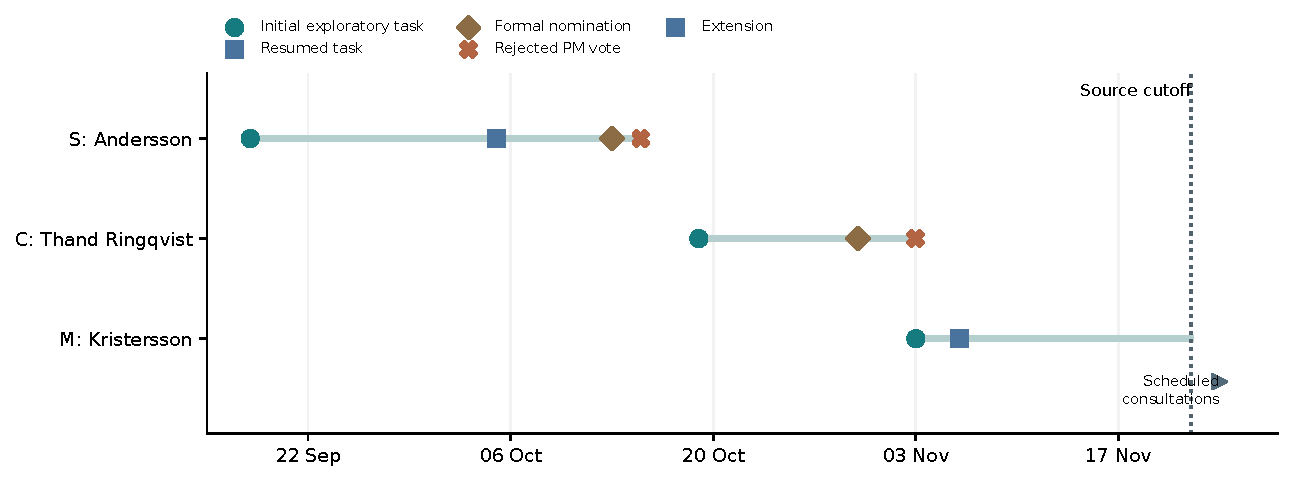
\includegraphics[width=\linewidth,height=.30\textheight,keepaspectratio]{process-chronology.pdf}
\caption{Documented formation sequence. Exploratory assignments, resumptions and extensions are distinguished from two rejected formal proposals. The 24 November event is a scheduled consultation and report, not an announced investiture ballot.}
\label{fig:chronology}
\end{figure}

Describing every extension as another rejected government inflates the formal failure count. Describing only the ballots discards the organisation of the preceding search. The ledger retains both, without assigning a final outcome to the unfinished M assignment. The 6 November Speaker notice also states that other parties can continue negotiating alongside an exploratory assignment; exploration is not coded as an exclusive bargaining monopoly.

\subsection{Election and investiture observations}

The versioned 2026 election dataset contains 29 constituencies, 124 party identifiers, 3,596 constituency--party vote cells and 6,767,429 valid votes. Constituency totals and quotas are retained. The parliamentary seat vector is shown in Table~\ref{tab:seats}. Source hashes identify the exact version; votes outside the intervention set remain in eligibility denominators \citep{val2026results}.

\begin{table}[tbp]\centering
\caption{Versioned 2026 parliamentary seats.}\label{tab:seats}
\begin{tabular}{lrrrrrrrr}\toprule
Party&S&M&SD&V&C&KD&MP&L\\\midrule
Seats&99&70&62&30&25&22&22&19\\\bottomrule
\end{tabular}
\end{table}

Official investiture notices provide observed party and member totals. Andersson's proposal received 99 Yes, 248 No, no abstentions and two absences, one each from V and MP. Thand Ringqvist's proposal received 25 Yes, 324 No, no abstentions and no absences \citep{riksdagAndersson,riksdagRingqvist}. These are two candidacies within one formation episode, not two independent electoral observations.

The source inventory distinguishes national party conditions, local disagreement and anonymous reported offers. A condition on cabinet participation is not automatically a future No vote. Candidate-specific future actions remain unknown in the documentary layer. Simulations use source-inspired assumption variants stated below; they do not relabel those variants as observed decisions.

\subsection{Ordinary parliamentary actions}

The parliamentary corpus contains all 2,612 recorded roll calls in four versioned session archives, 2022/23 through 2025/26 \citep{riksdagRollcalls}. Recounting the four included official archives reconciles 911,588 member records to 349 actions in every roll call. Independents' 8,035 actions are retained as observed Yes, No, abstention or absence. There are 897 reports, sixteen named committee labels including joint UF\"oU, and three records with an unclassified committee and missing date. Empty source dates are retained as missing values.

The corpus supplies two diagnostics. Exact action counts identify proximity to a declared intervention boundary. Party action profiles show whether an alignment persists after accounting for action frequencies and committee--session context. Neither turns an ordinary legislative vote into an investiture vote. The legal rule and final policy meaning of every record have not been classified; sensitivity is therefore a simple-majority counterfactual on the recorded balance.

These records examine recurring actions more broadly than two investiture observations permit. They also provide a negative comparison: parties can display persistent agreement on ordinary motions while taking different positions toward a candidate or cabinet. Statistical similarity and documentary commitment remain separate inputs.

\section{Exact response tensors}

\subsection{Representation as a composition of operators}

Let \(v_{dp}\) be votes cast for party \(p\) in constituency \(d\). An intervention \(u\) produces a nonnegative integer table \(v+u\), conserving each constituency's valid-vote total. The full electoral operator
\[
\mathcal A(v+u)=a(u)
\]
returns the national seat vector under the period-specific rule. Sweden's current modified Sainte-Lagu\"e sequence starts at \(6/5\), followed by 3, 5, 7 and subsequent odd divisors. The national threshold, regional exception, returned fixed seats and levelling seats are implemented by the complete procedure \citep{valmyndigheten,vallag}. Exact comparisons and typed unresolved cases prevent a tie from being silently resolved by party order.

For fixed local eligibility and quota \(K_d\), quotients \(Q_{dps}=v_{dp}/D_s\) admit a binary selection mask \(M\). Seats are counted by \(\sum_sM_{dps}\), with \(\sum_{p,s}M_{dps}=K_d\). The sum of selected quotient magnitudes is not a seat count. This tensor represents one allocation stage; it does not replace the national procedure.

Let \(N\) be an explicitly supplied set of parties that do not vote No. Under cohesive parties and full participation,
\[
g(u;N)=\sum_{p\in N}a_p(u),\qquad
y(u;N)=\ind\{g(u;N)\ge175\}.
\]
The electoral experiment fixes \(N=\{M,KD,L,SD\}\), a hypothetical template with 173 baseline seats. This supplies a representational boundary independently of those parties' future actions. The bargaining model subsequently uses the complete seat vector and its own action rules.

The response tensor indexes interventions:
\[
\mathcal T_{h,d,j,k}
=f\!\left(\mathcal A(v+u_{h,d,j,k})\right).
\]
The axes are ordered as direction pair \(h\), intervention constituency \(d\), first amount \(j\) and second amount \(k\), matching the recorded \(6\times29\times6\times6\) array. A separate mask records whether the inputs and required calculations are valid. Rejected inputs, changed eligibility and unresolved allocations remain unavailable, not zero.

\subsection{Six paired-transfer experiments}

Four disjoint directions are specified:
\[
\mathrm{MP}\to\mathrm{SD},\quad
\mathrm{S}\to\mathrm{M},\quad
\mathrm{V}\to\mathrm{KD},\quad
\mathrm{C}\to\mathrm{L}.
\]
The four directions cover each of the eight parliamentary parties once and move votes towards the fixed nonrejecting template. Disjoint donors and recipients make direct transfer costs additive. Their six unordered pairs are crossed with all 29 constituencies. Each amount takes one of six levels:
\[
\mathcal L=\{0,\ 2000,\ 5000,\ 10000,\ 15000,\ 20000\}.
\]
The resulting shape has \(6\times29\times6\times6=6264\) coordinates. The six levels provide a coarse design spanning no intervention through 20,000 voter changes per direction, with denser coverage near zero. The expanded design was fixed before its computations; these levels do not establish an optimal search resolution. Identical vote tables are computed once, including the zero intervention.

Donors and recipients are distinct within each pair. The net within-constituency half-\(L_1\) cost is consequently \(a+b\). Capacity is checked against the unchanged baseline before either transfer. Every valid table is allocated using all constituencies. Seats must sum to 349, constituency totals must remain fixed and admitted eligibility must be unchanged.

For an output \(f\), the anchored mixed difference is
\[
\Delta_{ab}f=f(a,b)-f(a,0)-f(0,b)+f(0,0).
\]
We calculate it separately for \(g\) and \(y\), requiring all four corners. A negative seat difference means that adding the separate gains overstates the joint gain. A positive threshold difference means that neither intervention reaches the boundary alone but their combination does, given this baseline. Threshold complementarity can occur with zero mixed seat difference because the threshold is another discontinuous operator.

The design is a finite counterfactual domain, not a random sample of elections. Counts of coordinates describe that domain. Moving the intervention constituency can alter capacity without altering the national target. We report both the response and where it is attainable. An axis named region is not, by itself, evidence of a regional effect.

\subsection{Member-action interventions}

For roll call \(r\), let \(Y_r,N_r,A_r,X_r\) denote Yes, No, abstention and absence counts, \(d_r=|Y_r-N_r|\), and \(W_r=\max(Y_r,N_r)\). Separate caps \(s,a,x\) permit winning-side switches, abstainers joining the trailing side and absentees returning for it. Strict reversal of the recorded balance is reachable exactly when
\[
R_{r,s,a,x}
=\ind\{2\min(s,W_r)+\min(a,A_r)+\min(x,X_r)>d_r\}.
\]
A switch changes the gap by two; a converted abstention or returning absentee changes it by one. Exact equality is separate. Baseline ties have no designated reversal direction; none occurs in this corpus.

Levels \(0,1,2,3,5,10,20\) define \(2612\times7^3=895916\) possible coordinates. The exact criterion permits evaluation on demand; the reported results use switch-budget profiles and specified joint-channel slices. Caps are separate: two switches and three returns permit five affected people. Joint responses are compared with single-channel corners. A signed difference of \(+1\) means both channels are needed at those caps; \(-1\) means each already suffices alone. Separate positive and negative counts prevent their cancellation from concealing both structures.

\subsection{Action associations without inferred commitments}

For each party and vote, the unique modal participating action is taken among Yes, No and abstention. A tied mode or no participation is missing. Weights \(w_r\) give each report equal total weight, divided among its usable votes. Let \(B_p\) denote party \(p\)'s modal participating action. For the pair-specific usable observations, define the normalised weight of session--committee cell \(c\) as \(W_c=\sum_{r\in c}w_r/\sum_rw_r\). The pair's observed agreement is compared with the independent-marginal reference using the same weights within session--committee cells:
\[
E_{pq}=100\left[
P_w(B_p=B_q)-\sum_cW_c\sum_bP_w(B_p=b\mid c)P_w(B_q=b\mid c)
\right].
\]
Excess agreement is in percentage points. It removes agreement implied by frequent use of the same action in the same recorded context. It does not match policy alternatives or establish coordination.

The first two sessions select three positive and three negative candidates with adequate common coverage. Their identities remain fixed for replay in the later sessions. All 28 pairs stay visible. Report-cluster resampling, exclusion of near-unanimous votes and leave-one-committee-out checks assess stability. Later-session results were already seen during development, so replay is retrospective.

\section{A finite-state model of formation}

\subsection{Proposal compatibility}

The process model asks whether an S-led proposal can be acceptable under explicit variants of composition conditions, policy assent and external tolerance. S is required in the cabinet; C, V and MP can enter or stay out, giving eight compositions. This restricted proposal family isolates one documented bargaining problem without claiming to enumerate every possible government.

A substantive state contains three policy-assent bits \(p_C,p_V,p_{MP}\) and two composition-release bits \(r_C,r_V\), giving \(2^5=32\) states. A policy bit records whether a package meets the modelled requirement. A release bit removes a specified composition condition. Neither is an estimated utility or ideological distance.

S supplies its seats to the nonrejecting side. C and MP tolerate the proposal when their policy condition is met. C also applies its composition condition when V is in the cabinet and C's requirement remains active. V's modelled participation demand applies when its nonrejection is necessary, holding the other modelled actions fixed. Let \(b_{-V}\) denote the number of nonrejecting seats excluding V. V is pivotal when
\[
b_{-V}<175\le b_{-V}+a_V.
\]
If V is pivotal, remains outside the cabinet and has not released its participation demand, its modelled action is No. Its policy-assent condition is separate. Cabinet consent is checked independently for each proposed member. A proposal can pass the numerical test while failing cabinet consent.

The source-to-rule mapping is explicit. C's 16 November statement requires V to release its cabinet-entry demand and both V and MP to back the proposed package \citep{cCondition}. V's platform combines a participation demand when its votes are needed with broader refusal wording \citep{vPlatform,vPlatformReadable}. The baseline model isolates composition conflict by treating policy assent separately and completing V's nonpivotal action as abstention. The cabinet predicate is an exclusion proxy for the participation-demand condition. These are analytical choices rather than uniquely determined future ballots. Table~\ref{tab:coding} records the choices and the alternatives tested. Budget support remains a distinct, unfilled variable.

\begin{table}[htbp]\centering\small
\caption{Statements, baseline predicates and alternative completions. Policy assent is a model state, not an observed prime-minister vote.}\label{tab:coding}
\begin{tabularx}{\linewidth}{>{\raggedright\arraybackslash}p{.22\linewidth}YY}\toprule
Source or design choice & Baseline completion & Sensitivity completion\\\midrule
C: V's participation demand and cross-party package acceptance & V is outside the cabinet, or C's exclusion condition is relaxed; C's own policy condition is met & C additionally requires both V and MP policy bits\\
V: conditional participation demand and broader refusal wording & V's unreleased outside demand blocks tolerance when pivotal & V votes No outside the cabinet whenever its participation demand remains active\\
Unannounced candidate-specific actions & Completed from declared state predicates & Both party-rule alternatives are crossed\\
Outside tolerance and cabinet selection & Supplied buffer; all eight S-led compositions available & Held fixed to isolate rule completion\\\bottomrule
\end{tabularx}
\end{table}

External tolerance has four party-cohesive variants: none, L, KD, and L plus KD, with baseline weights 0, 19, 22 and 41. An integer-buffer sweep from 0 to 60 separately isolates arithmetic boundaries. Intermediate weights are synthetic capacities, not invented parliamentary parties. All other parties vote No in the model.

Let \(F(a,K,p,r,e)\) conjoin cabinet consent and nonrejection for seat vector \(a\), cabinet \(K\), policy and release bits \(p,r\), and external tolerance \(e\). The agreement tensor stores this response for every declared combination and preserves its component tests. Failure can therefore be attributed to rejection, cabinet refusal or both.

\subsection{Concessions and reachability}

An agreement exists statically when
\[
\Feas(a,e)=\{(K,p,r):F(a,K,p,r,e)=1\}
\]
is nonempty. A process begins at a specified state and restricts how it changes. Adding policy assent costs one unit; releasing a composition condition costs two. These are declared cost indices for sensitivity analysis, not measured political sacrifices. Four release families permit neither condition, C only, V only or both conditions to change. External tolerance is a separate exogenous scenario; its negotiation cost is not included in this internal concession index.

Let \(\rho\) index the permitted release family and \(E_\rho\) the corresponding nonnegative-cost transition edges. Cabinet reconfiguration within the eight-composition family is freely available and unpriced. The distance measures policy and composition-clause changes; it excludes the cost of selecting a different cabinet and obtaining outside tolerance. The target graph states are the projection
\[
\States_F(a,e)=\{(p,r):\exists K,\ F(a,K,p,r,e)=1\}.
\]
For initial state \(s_0\), define
\[
\tau_\rho(a,e,s_0)=
\min_{\substack{\pi:s_0\leadsto_\rho s\\s\in\States_F(a,e)}}
\sum_{(u,v)\in\pi}c(u,v).
\]
If no permitted path exists, set \(\tau_\rho=\infty\). A budget \(B\) permits agreement exactly when \(\tau_\rho\le B\). We enumerate all eight initial policy combinations, release families and budgets 0 through 8. Static existence somewhere in the full state space, unrestricted-budget path existence under \(E_\rho\), and budget-limited reachability are different properties. The program's \texttt{structural\_possible} field denotes the second: a permitted path to a target, without the budget cap, not mere nonemptiness of the full agreement tensor.

A change of formateur that leaves the agreement set and transition graph unchanged cannot create a previously absent path. It can change which accessible proposals are examined first. A successful formateur-rotation claim must therefore identify an agenda change, another permitted transition or additional search resources. Repetition of an unchanged state is an explicit null control.

\subsection{Proposal agendas and the rejection horizon}

The eight cabinet compositions admit \(8!\) orders, all of which are enumerated. To isolate composition and agenda effects, the process runs start with all three policy conditions met, both composition conditions active, and a release budget of two units. The formal-testing protocol submits proposals in agenda order. An exploratory-only control instead evaluates proposals without submission. Exploratory search does not itself increase the formal-rejection counter. Submission of a numerically rejected proposal does. The process distinguishes a consented nonrejected proposal, exhaustion of four rejected proposals, and a proposal that is numerically nonrejected but lacks cabinet agreement. The last category uses a formal vote without adding a rejection and is not classified as a formed government.

Pressure-sensitive variants make one composition release available after \(k=1,2,3,4\) failed formal votes. The fourth rejection ends the procedure before a subsequent concession can rescue it. The fixed-agenda variant continues through the remaining proposals after a release. An exhaustive re-search control instead inspects the complete declared proposal family after release and identifies an acceptable proposal before another submission. It is a full-information upper benchmark for revisiting a proposal, not an estimated learning process.

Whole-episode experiments begin with zero rejected proposals. A distinct cutoff experiment begins with two, reflecting the two observed failures by 22 November and leaving two formal rejection slots. Neither count is advanced by adding an exploratory extension. Agenda frequencies describe the enumerated orders, not the likelihood of each order being selected by Swedish actors.

\subsection{Coupling representation and negotiation}

Complete seat vectors from the electoral tensor enter the process model after deduplication. For each distinct vector we recompute nonrejection, compatible cabinets, minimum concession cost and external-tolerance requirements. This links representation to agreement without claiming that vote shifts teach the model the parties' future actions.

The coupling can reveal a change in kind. If the S/C/V/MP family has at least 175 nonrejecting seats, an internal composition release may suffice. If it falls below 175 under the outsider-No variant, internal concessions cannot provide missing external seats. At least one outsider must change its modelled action. With party-cohesive options, this may mean an entire party rather than one member.

An electoral coordinate therefore determines a seat vector; that vector constrains agreement states; a transition rule determines paths to those states. The resulting objects are conditional interventions and obstructions, rather than a single score of political closeness.

\section{Results}

\subsection{A majority without common investiture support}

The S/C/V/MP total was 176 seats, but the observed ballots did not supply a common nonrejecting set on either candidate. On 15 October C's 25, V's 29 participating and MP's 21 participating members voted No to the S candidate. On 3 November S, V and MP voted No to the C candidate. A seat-only grouping therefore differed from the observed action configuration on both occasions.

Let \(N_{\No}\) denote the observed number of No votes. The individual No-to-abstention boundary is
\[
k_{\No\to\mathrm{abstain}}=\max(0,N_{\No}-174).
\]
It equals 74 in the first ballot and 150 in the second. One fewer leaves 175 No votes and preserves rejection. The Yes count need not increase. If each party's observed No voters must move together, minimum changed-member totals become 75 and 151. The first minimum comprises V's 29, C's 25 and MP's 21. One second-ballot witness is M's 70, SD's 62 and L's 19. Minimising the number of party groups is different: two can suffice, but with a different changed-member total.

\begin{table}[tbp]\centering
\caption{Observed 2026 ballots and retrospective No-to-abstention boundaries.}\label{tab:observed}
\begin{tabularx}{\linewidth}{Xrrrrrr}\toprule
Candidate and date&Yes&No&Abstain&Absent&Individual&Party-group\\
&&&&&boundary&boundary\\\midrule
Andersson, 15 October&99&248&0&2&74&75\\
Thand Ringqvist, 3 November&25&324&0&0&150&151\\\bottomrule
\end{tabularx}
\end{table}

The chronology shows why the episode cannot be reduced to failed ballots. A resumed exploration, a report, an extension and an adjournment change the organisation or timing of search. They do not increment the formal rejection count. At the cutoff, two rejection slots had been used, while M's exploration was unresolved. The simulations below keep the whole-episode horizon distinct from the remaining horizon at that date.

\subsection{Joint interventions are not interchangeable}

Figure~\ref{fig:tensor} summarises the mixed responses. The expanded experiment retains 4,931 distinct native input records for 6,264 coordinates; 2,685 are completed unique valid tables. There are 3,684 valid joint allocation coordinates and 2,580 donor-insufficient masks. Among 4,350 coordinates with both amounts positive, 2,271 have four complete corners and 2,079 are masked. The complete interior comparisons yield 233 negative seat differences, 2,010 zeros and 28 positive differences. Threshold differences are positive in 418 comparisons and zero in 1,853; none is negative in this domain.

\begin{table}[tbp]\centering\small
\caption{Exact results for all six transfer pairs. Four-corner counts concern positive-amount interior coordinates.}\label{tab:pairs}
\begin{tabularx}{\linewidth}{Xrrrrr}\toprule
Paired directions&Valid joint&Complete&\(\Delta g<0\)&\(\Delta g>0\)&\(\Delta y>0\)\\
&&four corners&&&\\\midrule
MP\(\to\)SD; S\(\to\)M&638&388&74&0&73\\
MP\(\to\)SD; V\(\to\)KD&501&296&24&0&76\\
MP\(\to\)SD; C\(\to\)L&487&286&22&0&72\\
S\(\to\)M; V\(\to\)KD&758&488&48&28&75\\
S\(\to\)M; C\(\to\)L&734&468&44&0&67\\
V\(\to\)KD; C\(\to\)L&566&345&21&0&55\\\midrule
Total&3684&2271&233&28&418\\\bottomrule
\end{tabularx}
\end{table}

The original MP-to-SD/S-to-M experiment is replicated exactly: 638 valid joint cells, 388 complete interior comparisons, 74 negative seat interactions and 73 positive threshold interactions. The expanded directions also produce a contrasting case that the original pair did not contain. In Stockholm, 5,000 S-to-M transfers alone leave \(g=173\), as do 5,000 V-to-KD transfers alone, but their combination yields \(g=174\). Here \(\Delta g=+1\), while \(\Delta y=0\). Superadditive representation need not cross the investiture boundary.

The reverse distinction also occurs. A 5,000 MP-to-SD transfer and 20,000 S-to-M transfers each give 174 separately and 175 together. Seats are additive at these four corners, \(\Delta g=0\), while threshold acceptance is complementary, \(\Delta y=+1\). The two results show why a single interaction label is insufficient: the response variable must be specified.

The beneficiary can also differ from the recipient. In Stockholm, 5,000 MP-to-SD transfers alone move M from 70 to 71 seats, MP from 22 to 21 and leave SD at 62. M receives no votes in that intervention. Across the 2,684 distinct valid nonzero electoral inputs, 494 have a seat gain for at least one party receiving neither transfer. This diagnostic can overlap with a gain to a recipient; it is not a partition into exclusive types.

Equal total voter cost does not fix the result. With 20,000 V-to-KD transfers alone, the target set has 174 seats. With 5,000 MP-to-SD and 15,000 V-to-KD transfers it has 175, at the same 20,000-voter cost. At 25,000 voters in the original pair, 10,000 MP-to-SD plus 15,000 S-to-M yields 174, whereas 15,000 MP-to-SD plus 10,000 S-to-M yields 175. Composition, not just intervention magnitude, determines the response.

\begin{figure}[tbp]\centering
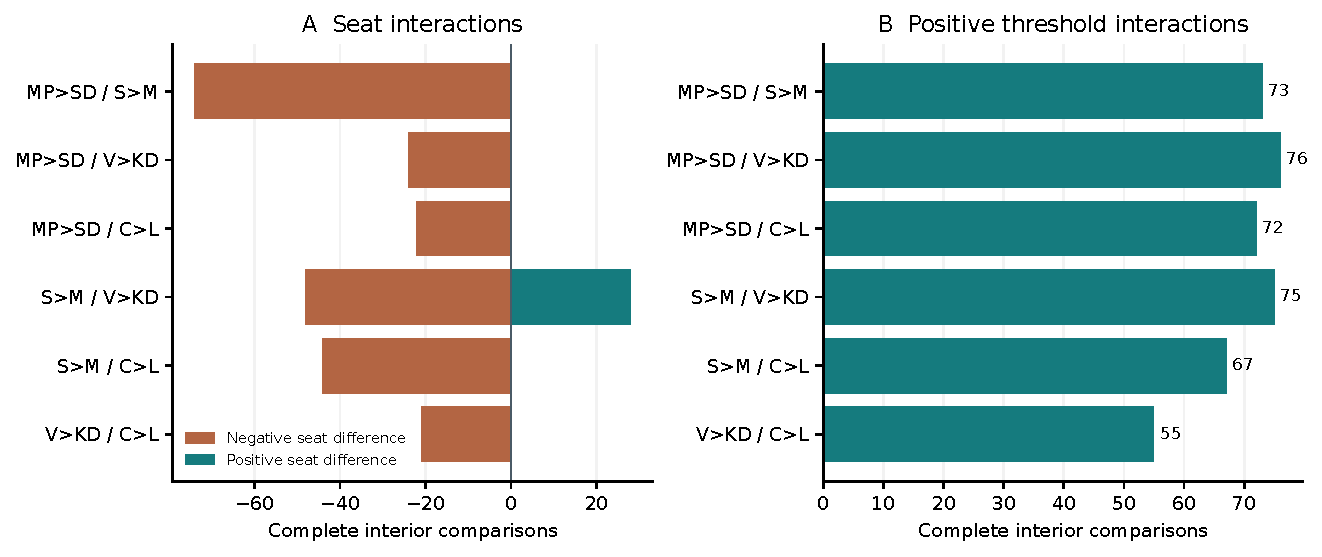
\includegraphics[width=\linewidth,height=.34\textheight,keepaspectratio]{tensor-interactions.pdf}
\caption{Exact paired-transfer responses in the versioned 2026 election data. Seat-count and threshold interactions are separate. The design crosses six direction pairs, all constituencies and the prespecified amount levels; unavailable four-corner comparisons remain masked.}
\label{fig:tensor}
\end{figure}

Two further results delimit the response. First, the smallest sampled successful cost falls from 25,000 in the original pair to 20,000 when directions expand. This is a grid minimum, not a global optimum. Second, for fixed direction pair and amounts, all completed constituencies give the same \(g\) in this design. Capacity masks differ geographically; an additional regional difference in this national target does not appear. The complete allocations produce only 26 distinct eight-party seat vectors: one with \(g=173\), ten with \(g=174\) and fifteen with \(g=175\). The coupling analysis therefore uses these 26 distinct vectors.

\subsection{Agreement, concession and accessible paths}

Figure~\ref{fig:bargaining} connects agreement constraints, costs and timing. The agreement experiment separates the absence of compatible proposals from the cost and sequence of reaching them. Its exhaustive tables retain every policy state, cabinet composition, release family, external buffer and declared budget.

\begin{figure}[tbp]\centering
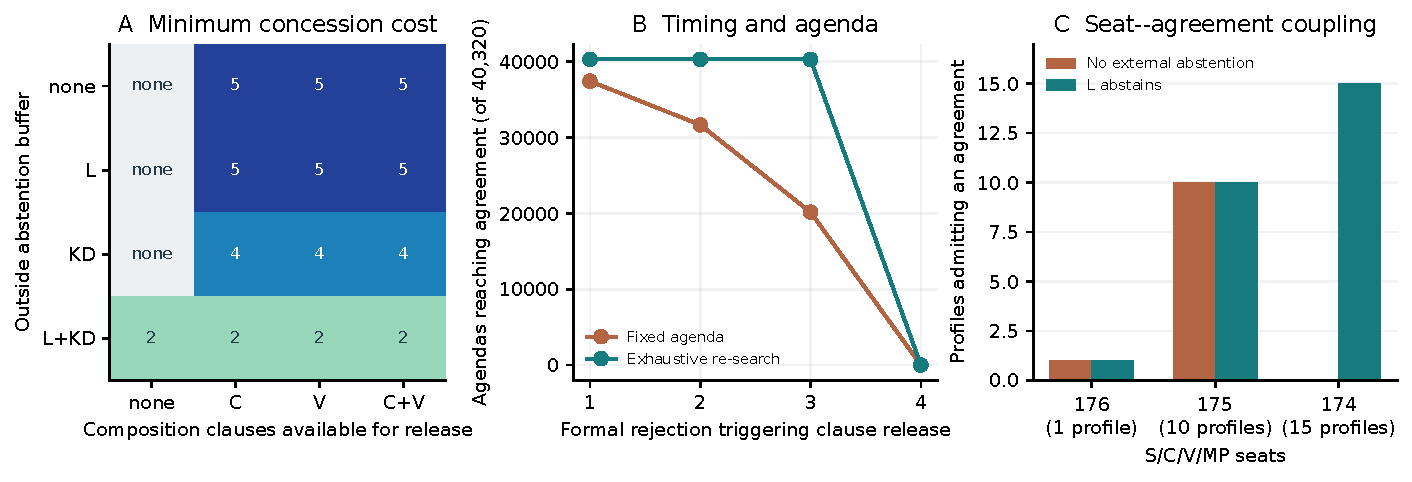
\includegraphics[width=\linewidth,height=.34\textheight,keepaspectratio]{bargaining-sensitivity.pdf}
\caption{Baseline-completion agreement states under composition releases, policy assent, external tolerance and finite proposal horizons. Frequencies refer to the specified enumerations, not the likelihood of a future Swedish cabinet.}
\label{fig:bargaining}
\end{figure}

The complete design contains 26,624 proposal evaluations, 29,952 reachability rows and 9,568 process settings. These are exhaustive combinations of declared inputs. Twenty-six seat profiles, rather than thousands of different political episodes, underlie the coupled results.

At the baseline seat vector, the two active composition conditions block every consented nonrejected S-led cabinet when outsiders vote No. The obstruction follows from the two composition conditions. Excluding V leaves its necessary tolerance conditional on cabinet entry; including V activates C's exclusion condition. Meeting all three policy conditions leaves this conflict in place. Either composition release removes the obstruction. Starting with no policy conditions met, the minimum path costs five: three policy-assent units and a two-unit composition release. Permitting both releases does not reduce this minimum because releasing either one already suffices.

\begin{table}[tbp]\centering
\caption{Minimum concession cost from policy state \(000\), baseline seats and baseline action completion. Policy assent costs one per party and a composition release costs two. A dash denotes no permitted path. External parties abstain as a declared scenario.}
\label{tab:cost}
\begin{tabular}{lrrrr}
\toprule
External tolerance & No release & C release & V release & Either permitted\\
\midrule
None & -- & 5 & 5 & 5\\
L (19 seats) & -- & 5 & 5 & 5\\
KD (22 seats) & -- & 4 & 4 & 4\\
L and KD (41 seats) & 2 & 2 & 2 & 2\\
\bottomrule
\end{tabular}
\end{table}

External tolerance changes the path's content, not merely its margin (Table~\ref{tab:cost}). L's 19 seats do not remove the composition obstruction or reduce the baseline five-unit path. Under independent policy bits, KD's 22 seats still do not solve strict composition incompatibility, but once either condition is released they can replace the MP policy-assent step: S, C and V plus KD have 176 seats. The minimum falls to four. With L and KD both abstaining, two policy conditions suffice without either composition release. For example, S, V and MP plus this buffer have 192 nonrejecting seats. The strict-composition minimum in a sweep that increases anonymous external tolerance one seat at a time is 24, so neither L nor KD alone reaches it. This is a conditional numerical threshold, not a claim that an arbitrary 24 members would act together.

The cost index can be varied without changing the existence result. With each policy unit held at one and a composition release priced at one, two or three, the no-external route costs four, five or six. The strict-condition obstruction survives all three prices because cost cannot create a transition that the release family prohibits. This separates a high-price path from an absent path.

The electoral coupling identifies a sharper boundary (Table~\ref{tab:coupling}). Of the 26 exact seat vectors, one leaves S/C/V/MP at 176 seats, ten leave it at 175, and fifteen at 174. Under outsider No, a permitted composition release and policy assent can produce agreement for the first eleven vectors. They cannot do so for the remaining fifteen, even when both composition releases are allowed. Internal agreement among 174 seats still leaves 175 No votes outside the family. A change from 175 to 174 thus changes the required \emph{kind} of cooperation: an external action becomes necessary. Allowing L tolerance restores a five-unit path in all 26 profiles; allowing both L and KD restores a two-unit path without composition release in all 26. KD alone yields cost four in 22 profiles and five in four, showing why the complete party vector carries information beyond a family total.

\begin{table}[tbp]\centering
\caption{Seat changes and the type of agreement required. Distinct vectors receive one count each; the rows are not outcome probabilities. Costs start at policy state \(000\).}
\label{tab:coupling}
\begin{tabular}{lrrr}
\toprule
S/C/V/MP seats & Distinct vectors & Internal release can suffice & External action necessary\\
\midrule
176 & 1 & 1 & 0\\
175 & 10 & 10 & 0\\
174 & 15 & 0 & 15\\
\bottomrule
\end{tabular}
\end{table}

Agreement existence does not determine whether a proposal sequence reaches it. Under unchanged composition conditions, every one of the \(8!=40{,}320\) baseline agendas exhausts four formal rejections. Making either C's or V's composition condition releasable after a formal failure opens a path, but the time of release and the unexamined agenda matter. Release after the first rejection yields 37,440 completed agreements; after the second, 31,680; after the third, 20,160. Release after the fourth yields none, because the rejection horizon has already ended (Table~\ref{tab:agenda}). C and V releases have equal counts in this design, although the compatible cabinets differ.

\begin{table}[tbp]\centering
\caption{Timing of one composition release across all 40,320 baseline agendas. All policy conditions are initially met, outsiders vote No, and the initial formal-rejection count is zero. Exhaustive re-search is a full-information control.}
\label{tab:agenda}
\begin{tabular}{lrrr}
\toprule
Release after rejection & Fixed-agenda agreements & Fixed-agenda failures & Re-search agreements\\
\midrule
No release & 0 & 40,320 & 0\\
1 & 37,440 & 2,880 & 40,320\\
2 & 31,680 & 8,640 & 40,320\\
3 & 20,160 & 20,160 & 40,320\\
4 & 0 & 40,320 & 0\\
\bottomrule
\end{tabular}
\end{table}

The re-search result isolates a procedural obstruction. An acceptable cabinet exists after a timely release, and an exhaustive reconsideration can find it. A fixed agenda can leave too little room to test a remaining acceptable cabinet. The control jointly permits feasibility search and reconsideration; their separate contributions are not identified by this comparison. The control demonstrates how exhaustive selection can overcome agenda truncation under these rules.

Starting at the observed cutoff changes the counter, not the law. Two formal proposals have already failed, so only two rejection slots remain. If a composition release becomes available after the third total rejection, fixed continuation reaches agreement in 20,160 agendas; exhaustive re-search reaches it in all 40,320. Waiting until the fourth total rejection again gives zero. Twelve unchanged exploratory evaluations consume no formal rejection slots and change no agreement condition. Four unchanged formal submissions consume all four. A mere count of political meetings would collapse these different processes.

Conditional pivotality produces a completion-sensitive local response. Adding policy assent can increase opposition under the conditional pivotality rule. In an S-only cabinet with C and V's policy conditions met but MP's unmet, V is not pivotal and abstains. There are 195 No votes. Meeting MP's condition contributes 22 nonrejecting seats, but now makes V pivotal while V remains outside the cabinet with its participation condition active. V's 30 seats switch to No; opposition rises to 203. The net change is eight additional No votes despite an additional policy assent. This rule-derived feedback occurs in 64 of 2,560 baseline proposal-edge comparisons across the four external buffers.

The countercheck limits that finding precisely. Neither endpoint of this example is an agreement, and no allowed concession edge destroys an existing agreement anywhere in the 26-profile enumeration. Local numerical support is nonmonotone; the tested agreement predicate remains monotone. The mechanism is therefore activation of a conditional participation demand during an already unsuccessful negotiation, not the destruction of a government by an extra supporter.

\subsection{Which conclusions depend on the action completion?}

A sensitivity experiment crosses the baseline and strict V action rules with independent and package-linked C policy predicates. It evaluates 106,496 proposal coordinates, 13,312 minimum-cost settings and 119,808 budget rows. Its baseline reproduces the original 26,624 proposal evaluations and 29,952 reachability rows exactly. Package linkage uses declared policy bits; it does not make C's action a function of V's endogenous ballot, which would introduce a different simultaneous-decision model.

The change from an internally sufficient family to one requiring outside tolerance survives all four completions: eleven profiles admit an internal route and fifteen do not. The baseline no-buffer, L-buffer and combined L--KD costs remain five, five and two. The KD boundary changes. Requiring C's cross-party policy condition raises the minimum to five in all 26 profiles, rather than four in 22 and five in four. The four-unit result therefore depends on the independent-policy simplification.

The striking No-count response is also completion-sensitive. The baseline example is \(195\to203\); strict outside refusal by V makes it \(225\to203\). Package-linked C gives \(220\to203\), and combining both gives \(250\to203\). Strict V coding changes 2,232 No counts while preserving every proposal's consent, nonrejection and agreement indicators. The equivalence follows from whether the non-V parties already suffice, cannot suffice even with V, or make V pivotal. The full-policy agenda agreement counts consequently remain unchanged. Appendix~\ref{app:completion} gives the proof and comparison table. The robust finding is the agreement boundary; the opposition-increase example describes one action completion.

\subsection{Ordinary-vote boundaries and conditional alignment}

Figure~\ref{fig:parliament} shows the sensitivity and alignment profiles. Most ordinary roll calls are far from a small switch cap. The median strict-reversal requirement is 76 winning-side switches. Twenty records can be reversed by one, 118 by at most two, 152 by at most three and 163 by at most five. The last count is 6.24\% of votes and 6.04\% under equal-report weighting. Close balances are therefore not explained merely by giving every subvote of a long report full weight.

There is domain variation. At most five switches suffice in 26 of 221 education, 17 of 161 transport and 22 of 285 health/social-affairs votes, compared with five of 110 defence and five of 242 environment/agriculture records. The close-balance rate rises from 17 of 564 votes in 2022/23 to 90 of 798 in 2025/26. These are differences in the recorded agenda, not matched-policy effects of time or committee.

Joint resources reveal another structure. Two switches alone can reverse 118 records; three returning absentees alone can reverse 49; together they reach 154. Thirty-six records require both channels at those caps, while 49 are already reversible by either channel alone. The signed total, \(-13\), would hide the 36 complementary cases. In education record UbU21/4 on 4 June 2025, a 153/149 balance and 47 absences yield 151/151 after two switches, 153/152 after three returning No voters and 151/154 when the operations combine.

\begin{figure}[tbp]\centering
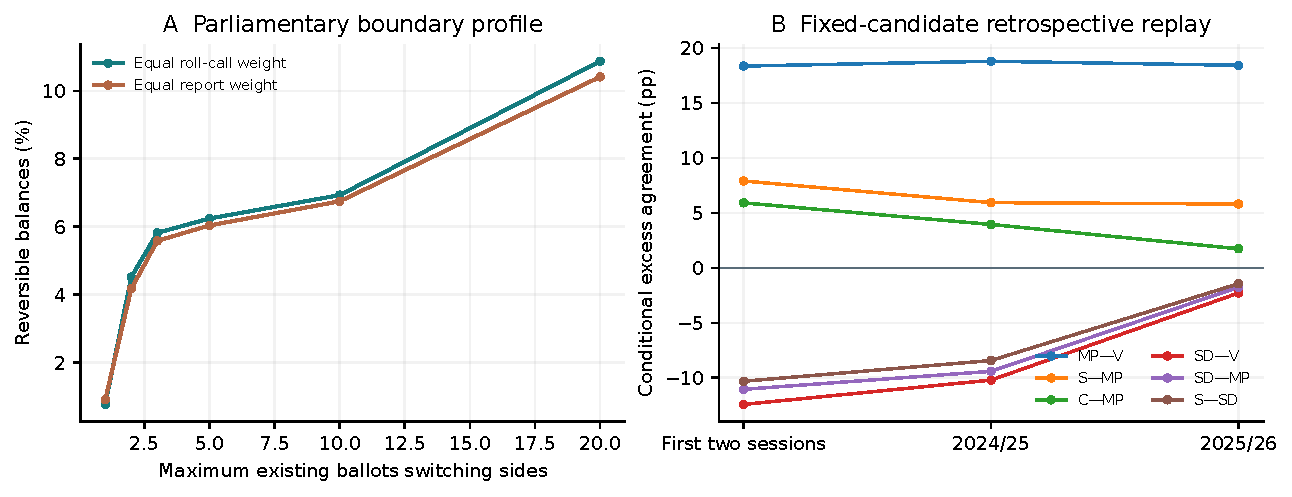
\includegraphics[width=\linewidth,height=.34\textheight,keepaspectratio]{rollcall-patterns.pdf}
\caption{Parliamentary sensitivity and conditional action patterns across four sessions. Report weighting and action-rate references use the same usable observations. Ordinary-motion agreement is not coded as cabinet or investiture consent.}
\label{fig:parliament}
\end{figure}

Conditional party associations sharpen the distinction. MP--V excess agreement is \(+18.36\) percentage points in the first two sessions, \(+18.80\) in 2024/25 and \(+18.43\) in 2025/26. Final-session observed agreement is 58.52\%, versus a 40.09\% conditional reference. Excluding near-unanimous votes leaves \(+18.29\); removing committees individually leaves \(+17.75\) to \(+19.35\). Within the recorded contexts, the relationship is not reduced to a common frequent action or one committee.

C--MP is a counterpattern: excess agreement falls from \(+5.92\) to \(+3.95\) and \(+1.74\), and later resampling ranges include zero. S--MP varies by topic, with \(+15.27\) points in education, \(+14.31\) in health/social affairs and \(-2.18\) in defence. M--SD offers another diagnostic: final-session raw agreement and its equal-report reference both equal 97.237\%, leaving zero excess under that reference. Very high raw agreement need not imply a residual association.

The recurring structure in ordinary actions does not identify the cabinet or candidate the same parties will accept. S--MP retains \(+5.81\) points of excess agreement in the final ordinary-vote session, yet on 15 October MP supplied 21 No votes and one absence to the S leader's candidacy. The contrast concerns different decisions: ordinary motions and a named prime-minister proposal. It rules out an automatic conversion of their alignment measures. The corpus offers a broad behavioural description, but it cannot substitute thousands of motions for additional government-formation episodes.

\subsection{Relation to the wider research programme}

The joint-transfer grid is one part of a larger programme. Earlier exact searches established conditional full-allocation minimum voter-change costs of 9,086 in 2022 and 10,269 in 2026 under a fixed eight-party domain. Their search domain is broader than the present six-level grid; a sampled 20,000-voter crossing is therefore compatible with the smaller domain-wide minimum. The earlier theorem and the present grid's four-vote correction guard have different validated scopes.

The programme also fitted CP and Tucker models, reconstructed full-period SVD geometry and examined seven historical elections for poll-to-election calibration. CP and Tucker reduced interpolation error in an initial single-class test, but a later two-class cross-election test favoured a simple quota comparator. The calibration panel improved some marginal error summaries while failing joint coverage in all three eight-party test elections. These results support keeping exact allocation at the decision boundary and treating learned reconstructions and calibrated stress scales as separate research objects. Appendix~\ref{app:programme} reports their values and provenance. These recorded results are supplementary data, separate from the five experiments reproduced here.

\section{Discussion}

The central result is the separation of arithmetic possibility, acceptable agreement and a path to agreement. A majority can be present in the seat vector while compatible proposals are absent under the modelled conditions. Compatible proposals can exist while the negotiation cannot reach them within its resources. A proposal can also be arithmetically nonrejected while a proposed member refuses cabinet participation. Each outcome has a different computational witness and political interpretation.

This changes how repeated assignments should be read. When rules and state are unchanged, another exploratory round cannot create a new compatible agreement. If formateur rotation succeeds in the model, the explanation must be a changed agenda, a newly permitted transition or additional search resources. When a rejection-sensitive concession opens a route, time alone is not the mechanism; the mechanism is the specified link between a formal event and a subsequent commitment. The Speaker's account makes that link a reasonable object of investigation while leaving its actual operation an empirical question.

Representation adds a connection omitted by static compatibility diagrams. The recipient of changed votes need not receive the changing seat; single effects need not add; a threshold can be complementary even when seats are additive. The resulting complete vector changes the negotiation problem. A small representational movement can remove an internally sufficient route and make external tolerance necessary. What must be explained is consequently not just how many seats change but what form of cooperation becomes required.

For computational sociology, the tensor's value is in retaining these joint conditions and exposing their margins. Unfolding it into a matrix is harmless if indices remain known. Aggregating away a cabinet condition, a proposal stage or an unavailable calculation is not. An axis acquires substantive meaning through its operation: who is included, whose assent is conditional, whether a party is pivotal and which event increments the rejection counter. The explanatory content lies in the actor-specific conditions and transition rules retained by the tensor.

The analysis also identifies observations needed to distinguish explanations of delay. Structural incompatibility predicts repeated failure until a blocking condition or external action changes. Restricted search predicts that an acceptable proposal existed but remained outside the explored path. Pressure predicts a change in the timing or accessibility of concessions after a specified event. Discriminating among these mechanisms requires records of proposals, counteroffers and decisions, not only the eventual cabinet and elapsed days. The event ledger is therefore part of the design rather than background to its numerical work.

Ordinary-vote results impose a further interpretive discipline. Persistent action relations make wholesale behavioural independence implausible as a description, but they do not identify a unique governing arrangement. Topic-dependent associations and candidate-specific rejections show why a relation measured on one object cannot transfer unchanged to another without a model. Such transfer can be assessed in a larger event archive; it is not established by the number of roll calls.

\section{Scope and validation}

The article separates three evidential levels. Official notices and ballots establish recorded events at dated cutoffs. Exact allocation and enumeration establish implications of the admitted inputs and rules. Process experiments investigate specified mechanisms; their agenda frequencies and concession costs are not estimates of Swedish actors' probabilities or utilities.

The election dataset is versioned. A publisher notice concerning four omitted small-party votes motivates an explicit input-correction check. The guard audits all 4,931 native records and proves invariance for the 2,685 completed unique valid tables. Adding at most four nonnegative votes solely to parties outside the original eligible eight, with quotas fixed, changes no eligible set or eligible-party quotient. All 3,684 completed tensor coordinates therefore retain their allocations. Appendix~\ref{app:allocation} supplies the gap bounds. This covers that stated correction class, not arbitrary data errors or a global minimum search. Turnout and quotas are otherwise fixed; only specified nationally eligible parties receive interventions; candidate-list capacity is not modelled. A finite grid covers neither every electoral change nor a global minimum.

The source cutoff is 22 November 2026. Retrieving an older page later does not establish that an identical version was available before an earlier decision. Conditional national statements, local statements and anonymous reports remain different claim types. There are only two completed formal ballots in the episode. Ordinary votes and counterfactual coordinates do not increase that number. Temporal replays and source reconstruction are retrospective rather than blind prospective validation.

The small bargaining model makes its paths checkable. It restricts the cabinet family, discretises assent and assigns explicit concession costs. Results concern those assumptions and their examined variations. Private information, endogenous utilities, rival candidate strategies and longer-term policy bargains require further observations and a different model. The exact finite design identifies consequences and counterexamples; it does not eliminate uncertainty about the mechanism operating in the historical episode.

Implementation checks include invariant recomputation, small-state enumeration, native replays and comparisons with stored numerical outputs. The repository contains source versions, protocols, complete tables and the commands for reproducing calculations.

\section{Conclusion}

Sweden's 2026 episode illustrates why parliamentary seat totals do not determine government formation. The relevant majority may exist numerically while the conditions for cabinet participation and investiture tolerance do not fit together. Even compatible agreements can remain inaccessible within the permitted sequence.

Exact response tensors make the representational side inspectable; a finite state graph makes the procedural side inspectable. Coupling them shows how changes in seats alter the type of cooperation required. Official investiture votes and the ordinary-vote census place those conditional results in a documented parliamentary setting. The resulting research object is an account of which interventions, commitments and paths can change a specified outcome.

\section*{Data and computation}
The repository contains the native allocation source, Python implementation, versioned inputs, event ledger, frozen protocols, complete JSON/CSV outputs and LaTeX sources. Core experiments use the Python standard library and Rust; figures use recorded plotting dependencies. Verification checks hashes, while reproduction recomputes experiments and compares stable numerical results. 

\clearpage
\appendix
\numberwithin{table}{section}
\numberwithin{equation}{section}
These appendices define the computational domains, prove the boundary results used in the article and record numerical checks. Repository paths identify the code and evidence for each calculation.

\section{Computational contract and units}

The project contains five numerical experiments: exact paired voter transfers; finite-state cabinet compatibility and proposal sequences; member-action sensitivity and party-action associations; a bounded input-correction guard and party-action completion sensitivity. They share versioned inputs but retain different observational units.

\begin{table}[htbp]\centering
\caption{Objects retained by the experiments. A coordinate is a model combination, not an independent observed political event.}
\begin{tabularx}{\linewidth}{l r X}
\toprule
Object & Count & Interpretation\\
\midrule
Recorded parliamentary roll calls & 2,612 & Ordinary member-action records in four sessions\\
Member-action rows & 911,588 & 349 actions per recorded roll call\\
Distinct parliamentary reports & 897 & Clusters used for weighting and resampling\\
Completed 2026 PM ballots & 2 & Two proposals within one formation episode\\
Electorate tensor coordinates & 6,264 & Pair, constituency and two amount indices\\
Distinct native input records & 4,931 & Includes requests failing donor capacity\\
Completed unique valid tables & 2,685 & Deduplicated completed allocations, including baseline\\
Complete interior contrasts & 2,271 & Four valid corners with both amounts positive\\
Distinct complete seat vectors & 26 & Inputs to the formation experiment\\
Formation proposal coordinates & 26,624 & Profile, buffer, state and cabinet combinations\\
Reachability rows & 29,952 & Initial states, release families and declared budgets\\
Process settings & 9,568 & Profiles, buffers, horizon and pressure configurations\\
\bottomrule
\end{tabularx}
\end{table}

The transfer protocol crosses six direction pairs, 29 constituencies and six levels on each amount axis. There are \(6\cdot29\cdot5^2=4350\) positive-amount interior coordinates. Of these, 2,079 lack a completed four-corner comparison. There are 2,580 masked joint coordinates in the entire grid; all fail donor capacity in the observed run. A masked value is stored with a reason and a null numerical response. It never contributes a zero effect to a histogram. Frozen protocols identify the exact expanded computation; they are not independent preregistration. Baseline cases and later-session records had already been examined during development.

The response tensors in the present experiments are exact indexed objects; missing responses are not supplied by low-rank reconstruction. Earlier CP and Tucker fits from the wider research programme are summarised in Appendix~\ref{app:programme}. The party-action analysis estimates explicitly defined conditional associations, rather than treating tensor factor loadings as commitments. A matrix unfolding would retain the same information if every index and mask were preserved.

\section{Allocation, interventions and input correction}\label{app:allocation}

\subsection{The allocation operator}

The native engine receives all 29 constituency tables, 124 party identifiers and the fixed constituency seat quotas. It uses the current rule version, selected explicitly by election year. The 2026 packet contains 6,767,429 valid votes. Votes of parties outside the intervention set remain in the threshold denominators.

For national party votes \(V_p\), total valid votes \(T\), constituency votes \(v_{dp}\) and constituency total \(D_d\), national eligibility is
\[
100V_p\ge4T.
\]
The constituency exception uses \(100v_{dp}\ge12D_d\). A locally eligible party outside the national set is not simply assigned national levelling seats. The native procedure first allocates fixed seats, computes the appropriate national entitlement, returns and reallocates fixed awards where the current law requires it, and places levelling seats. A constituency quotient tensor alone therefore does not implement the complete Swedish allocation.

The first divisor is \(6/5\), followed by \(3,5,7,\ldots\). Rational comparison is performed by cross multiplication in a wider integer type. The relevant first quotient can be represented by numerator \(5v\) and denominator 6. A selected quotient counts one seat regardless of its numerical magnitude. The engine returns a typed tie rather than resolving it by an undocumented party order. Its protected-overhang exception is also explicit. Such unresolved cases would remain outside a completed response, rather than being assigned a convenient result.

Each paired intervention changes four distinct party cells in one constituency:
\[
u_{d,p_1}=-a,\quad u_{d,q_1}=a,\quad
u_{d,p_2}=-b,\quad u_{d,q_2}=b.
\]
The source capacities are checked on the unchanged baseline. Nonnegativity, constituency totals, national valid-vote total, eligible-party identities and the chamber total are then checked. Because the two directions have disjoint endpoints,
\[
\frac12\sum_{d,p}|u_{dp}|=a+b.
\]
This equals the number of voters reassigned under the declared direct-transfer interpretation. A design allowing overlapping paths or voter circulation would require another accounting rule.

Native input records are deduplicated before allocation; zero interventions and identical tables shared by direction pairs do not become separate computations. The full coordinate map remains in the tensor, so response frequencies can still be stated for the prespecified design. Recipient and nonrecipient gains are instead counted on unique nonzero valid tables.

\subsection{A bounded correction theorem}

The source publisher reported four omitted small-party votes. The correction guard tests the class of at most four nonnegative additions to parties outside the original eight nationally eligible parties, in any admitted constituencies, with fixed seat quotas and no correction to an eligible party's votes.

Let \(k\le4\) denote total additions. Define the following scaled eligibility gaps:
\[
G^{\rm in}_p=100V_p-4T,\quad
G^{\rm out}_p=4T-100V_p,\quad
H^{\rm out}_{dp}=12D_d-100v_{dp}.
\]
An inside party's gap loses at most \(4k\), because its votes do not change. An outside party receiving \(k_p\le k\) additions has outside-national gap change \(4k-100k_p\ge-96k\). In a constituency receiving \(k_d\) additions, the corresponding outside-regional change is \(12k_d-100k_{dp}\ge-88k\).

\begin{table}[htbp]\centering
\caption{Worst-case eligibility margins over all completed unique inputs. Positive residuals retain the admitted eligible set under the stated correction class.}
\begin{tabular}{lrrr}
\toprule
Gap & Minimum observed & Maximum loss & Residual\\
\midrule
Inside national & 9,048,984 & 16 & 9,048,968\\
Outside national & 23,105,316 & 384 & 23,104,932\\
Outside constituency & 482,812 & 352 & 482,460\\
\bottomrule
\end{tabular}
\end{table}

\begin{proposition}\label{prop:correction}
For every completed unique transfer input in the experiment, additions within the stated four-vote correction class leave its complete allocation unchanged.
\end{proposition}
\begin{proof}
The positive residual gaps retain all eight nationally eligible parties and exclude every outside party both nationally and under the regional exception. All eligible-party vote counts are unchanged. The fixed quotas, exact eligible-party quotients, national entitlement comparisons, returned-seat comparisons and levelling comparisons are consequently unchanged. The deterministic completed allocation is the same.
\end{proof}

The audit inspects 4,931 raw records and covers 2,685 completed unique valid tables, corresponding to 3,684 completed tensor coordinates. It does not supply a missing allocation for a donor-insufficient request. Nor does it cover vote removals, corrections to eligible parties, altered quotas or the recertification of an earlier global optimization claim. The protocol, gap witnesses, proof conditions and tests are in \path{results/input-correction/summary.json} and its manifest.

\section{Mixed differences and beneficiary diagnostics}

Let \(g_{ab}\) be the seat total of the declared nonrejecting template \(\{M,KD,L,SD\}\), and \(y_{ab}=\ind\{g_{ab}\ge175\}\). The anchored interaction is
\[
\Delta g=g_{ab}-g_{a0}-g_{0b}+g_{00};
\qquad
\Delta y=y_{ab}-y_{a0}-y_{0b}+y_{00}.
\]
The baseline is \(g_{00}=173\), \(y_{00}=0\). A seat effect and a threshold effect are not interchangeable. Even an additive seat response can cross a threshold only in the joint intervention.

\begin{table}[htbp]\centering
\caption{Completed four-corner witnesses in Stockholm. Amounts are direct voter transfers. All four corners use the full national allocation.}
\begin{tabular}{llrrrrrr}
\toprule
First direction & Second direction & \(g_{00}\)&\(g_{a0}\)&\(g_{0b}\)&\(g_{ab}\)&\(\Delta g\)&\(\Delta y\)\\
\midrule
MP to SD, 5,000 & S to M, 10,000 &173&174&174&174&$-1$&0\\
MP to SD, 5,000 & S to M, 20,000 &173&174&174&175&0&1\\
S to M, 5,000 & V to KD, 5,000 &173&173&173&174&1&0\\
\bottomrule
\end{tabular}
\end{table}

The first row demonstrates redundancy in seat gains; the second has threshold complementarity without a mixed seat effect; the third has a positive mixed seat effect without threshold success. All six direction pairs are reported in the article, including zero and opposite-sign cases. Across the complete interior, the seat-interaction histogram is \((-1:233,\ 0:2010,\ +1:28)\), while the threshold histogram is \((0:1853,\ +1:418)\).

For a beneficiary diagnostic, let \(R(u)\) be the set of direct recipients in the declared transfer and \(a_p(u)-a_p(0)\) each party's seat change. A nonrecipient gain is
\[
\ind\{\exists p\notin R(u):a_p(u)>a_p(0)\}.
\]
There are 494 such cases among 2,684 unique valid nonzero inputs. A recipient gain and a nonrecipient gain may coexist. The 1,072 inputs with no recipient gain include completely unchanged seat vectors; they cannot all be classified as gains to outsiders.

All 26 distinct complete eight-party vectors are retained for bargaining. At fixed pair and amounts, the target total has no additional constituency variation among valid entries in this design. This is a result on the sampled domain; it is not an assumption that constituency information may be dropped from other intervention families.

\section{Member-action boundary arithmetic}

Let \(d=|Y-N|>0\) be the initial Yes--No gap. A switch by one member from the winning to the trailing side decreases the gap by two. An abstainer joining the trailing side or an absent member returning for it decreases it by one. With separate caps \(s,a,x\), the largest possible decrease is
\[
C=2\min(s,W)+\min(a,A)+\min(x,X),
\]
where \(W=\max(Y,N)\). The operations use disjoint baseline action categories.

\begin{proposition}\label{prop:reversal}
Strict reversal is reachable under these separate caps exactly when \(C>d\).
\end{proposition}
\begin{proof}
No permitted person-level change reduces the original gap by more than its stated coefficient, so \(C\le d\) precludes a strict reversal. If \(C>d\), applying the permitted changes at their caps, with saturation at the available category counts, makes the new signed gap \(d-C<0\). This constructs a reversal.
\end{proof}

Thus a switch-only minimum is \(\lfloor d/2\rfloor+1\) when enough winning-side members exist. Equality \(C=d\) produces a tie rather than strict reversal. Baseline tied votes require a separate direction convention and are excluded from this reversal formulation; none occurs in the admitted corpus. The formula does not adjudicate substantive procedural exceptions applying to particular parliamentary motions.

The cap grid \(0,1,2,3,5,10,20\) on three axes defines 895,916 possible coordinates. The closed-form criterion evaluates them on demand; the recorded results retain switch-budget profiles and specified joint-channel slices rather than a materialised dense array. A two-channel mixed difference compares the joint cap with each single channel and the unchanged baseline. At caps \(s=2,x=3,a=0\), the joint response is reachable in 154 roll calls. Thirty-six require both channels, while 49 can already be reversed by either alone. The signed sum \(36-49=-13\) is therefore less informative than its two components.

\begin{table}[htbp]\centering
\caption{Ordinary-vote switch boundaries. Percentages weight each roll call equally.}
\begin{tabular}{lrr}
\toprule
Switch cap & Reversible roll calls & Roll-call percentage\\
\midrule
1&20&0.77\\
2&118&4.52\\
3&152&5.82\\
5&163&6.24\\
10&181&6.93\\
20&284&10.87\\
\bottomrule
\end{tabular}
\end{table}

An explicit education example is UbU21/4, 4 June 2025: 153 Yes votes, 149 No votes, no abstentions and 47 absences. Two switches reach 151--151; three returning No voters reach 153--152; the joint intervention reaches 151--154. This is complementarity between member-action resources, distinct from the electorate-allocation interactions.

\section{Conditional party-action associations}

For each party in each record, the action is the unique modal participating response among Yes, No and abstention. A tied mode, or no participating members, is missing. Absence is retained in member counts but is not treated as a participating policy action. Pair-specific usable observations are selected before computing either observed or reference agreement.

For report \(j\) with \(n_j\) usable pair records, each receives weight \(1/n_j\). Every usable report has total weight one. In session--committee cell \(c\), let \(W_c\) be its normalised total report weight and \(p_{pc}(b)\) the corresponding action marginal. The reference is
\[
P_0=\sum_c W_c\sum_{b\in\{Y,N,A\}}p_{pc}(b)p_{qc}(b).
\]
Observed agreement \(P_o\) uses exactly the same record selection and weights. Excess agreement is \(100(P_o-P_0)\), in percentage points; a normalised conditional kappa is also retained when \(P_0<1\).

This reference permits parties to have different action rates and permits those rates to vary by recorded context. It removes neither unrecorded subject matter nor the meaning of the proposed alternatives. It is a descriptive comparison with conditional independent margins, not identification of a latent alliance or a coordination effect.

The first two sessions, 2022/23 and 2023/24, select the three most positive and three most negative pairs among those with at least 40 common records, ten reports and defined conditional kappa. Ties are broken by pair identity. All 28 pairs qualify, and every pair remains visible in the inventory. The six selected identities are then replayed without replacement by later winners.

\begin{table}[htbp]\centering
\caption{Fixed candidate replay. Excess agreement uses equal-report weights and session--committee references. Final-column ranges are descriptive report-cluster resampling percentiles.}
\begin{tabular}{lrrrr}
\toprule
Pair & 2022/23--2023/24 & 2024/25 & 2025/26 & 2025/26 range\\
\midrule
MP--V &18.36&18.80&18.43&[14.47,21.49]\\
S--MP &7.91&5.94&5.81&[2.56,8.65]\\
C--MP &5.92&3.95&1.74&[$-1.92$,4.39]\\
SD--V &$-12.42$&$-10.21$&$-2.28$&[$-3.90$,$-0.96$]\\
SD--MP &$-11.05$&$-9.41$&$-1.75$&[$-2.95$,$-0.69$]\\
S--SD &$-10.31$&$-8.42$&$-1.44$&[$-2.23$,$-0.57$]\\
\bottomrule
\end{tabular}
\end{table}

Resampling draws reports with replacement within session--committee cells, preserving all usable votes in each selected report and assigning each report occurrence unit weight. The reference is recomputed in each replicate. There are 200 replicates with seed 20261122. The recorded percentile range is a stability diagnostic for this archive, not a population confidence interval or a prospective success rate.

Two further checks remove near-unanimous records using a .975 participating-majority cutoff and omit each committee in turn. MP--V retains 18.29 points after the first check and ranges from 17.75 to 19.35 under the second in 2025/26. C--MP's later ranges include zero. The negative pairs retain their sign but weaken substantially in the last session. These are different stability patterns, not a single conserved parliamentary partition.

The present party-action comparisons use the complete 2022/23--2025/26 corpus directly. Earlier full-period SVD results are summarised in Appendix~\ref{app:programme}. The reported full-period results are direct action counts, finite boundary responses and explicit pairwise conditional associations.

\section{The cabinet-state graph}

\subsection{State, roles and consent}

For a fixed seat profile \(a\), proposed cabinet \(K\) and external tolerance buffer \(e\), let the substantive state be
\[
s=(p_C,p_V,p_{MP},r_C,r_V)\in\{0,1\}^5.
\]
The implementation packs the first three bits as \(p_C+2p_V+4p_{MP}\). Release bits equal one when the corresponding condition is removed. S is always in the cabinet; any subset of C,V,MP may join. There are eight cabinets and 32 substantive states.

S is nonrejecting. C is nonrejecting if \(p_C=1\) and either V is outside \(K\) or \(r_C=1\). MP is nonrejecting if \(p_{MP}=1\). For V, compute the other parties' nonrejecting seats \(b_{-V}\) first, including the supplied external buffer. V's conditional pivotality is
\[
I_V=\ind\{b_{-V}<175\le b_{-V}+a_V\}.
\]
V is nonrejecting if \(p_V=1\) and at least one of the following holds: \(I_V=0\), V is in \(K\), or \(r_V=1\). A hopeless proposal with \(b_{-V}+a_V<175\) does not label V pivotal. A supporting cabinet member votes Yes; a supporting nonmember abstains. Other parties vote No unless specified in the external buffer.

The buffer options are none, L, KD and L+KD. They are exogenous action assumptions, not observed promises. Their acquisition costs are excluded from the internal concession index.

Cabinet consent is a different predicate. Every included party must meet its policy condition; included C must also satisfy its composition condition. Nonrejection requires fewer than 175 No votes. The agreement indicator is the conjunction of consent and nonrejection. Budget support is deliberately unfilled rather than imputed from either.

\subsection{Permitted changes and minimum costs}

Edges add a missing policy bit or release an active composition condition, as allowed by release family \(\rho\). Edges never retract assent or reactivate a condition. For policy unit cost \(c_p\) and release cost \(c_r\), path cost is the sum of edge costs. Cabinet reconfiguration itself is unpriced within the declared family. The principal setting is \(c_p=1,c_r=2\).

Let \(\States_F(a,e)\) be states admitting at least one consented nonrejected cabinet. For initial state \(s_0\),
\[
\tau_\rho(a,e,s_0)=
\min_{\pi:s_0\leadsto_\rho s,\ s\in \States_F(a,e)}
\sum_{(u,v)\in\pi}c(u,v).
\]
The minimum is infinity if no permitted path exists. Enumerating all states or using shortest paths gives the same result in this acyclic five-bit graph. The result field \texttt{structural\_possible} denotes finite \(\tau_\rho\), without a budget cap. It is not mere nonemptiness of \(\States_F\) when that set contains states reachable only under another release family.

Nine cost settings cross \(c_p,c_r\in\{1,2,3\}\). At the baseline from policy state \(000\), permitting either C or V release gives
\[
\tau_{\rho}=
\begin{cases}
3c_p+c_r,&e=\varnothing\text{ or L},\\
2c_p+c_r,&e=\text{KD}.
\end{cases}
\]
With both L and KD tolerating, the minimum is \(2c_p\) even with neither composition release permitted. If no release is permitted and the buffer is none, L or KD, the route remains absent for every price. These are additive indices, not ordinal utilities or measured political sacrifices.

\subsection{Conditional pivotality and monotone agreement}

For the baseline S-only cabinet, policy mask 3 means C and V assent but MP does not. V is not pivotal: others supply \(99+25=124\), and \(124+30<175\). It abstains, giving 195 No votes. Adding MP assent makes the others supply 146 nonrejecting seats. Now \(146<175\le176\), so V's unfulfilled cabinet-entry condition activates and its 30 seats move to No. No votes rise to 203. This local effect was identified during model development.

\begin{proposition}\label{prop:monotone}
Under the stated rules and fixed cabinet, seat vector and external buffer, adding a permitted policy assent or composition release cannot turn an existing agreement into a disagreement.
\end{proposition}
\begin{proof}
Non-V nonrejection and each cabinet-consent predicate are monotone in the allowed changes. The only possible withdrawal is V's, when increased assent by others activates its pivotal participation condition. If V is in the cabinet or its condition is released, that withdrawal is unavailable. Otherwise, an initial agreement with V outside and rigid must already have at least 175 nonrejecting seats excluding V: fewer would either leave the proposal hopeless or make V pivotal and unwilling. Other parties' nonrejection cannot fall, so they remain sufficient after the change. Consent also remains satisfied.
\end{proof}

The exhaustive edge diagnostic checks 66,560 fixed-cabinet proposal edges across 26 seat profiles and four buffers. It finds 1,424 edges increasing No votes and zero edges losing an agreement. The baseline contributes 64 No-increasing edges among 2,560. This checks implementation of the proposition while distinguishing local numerical nonmonotonicity from agreement loss.

\section{Sequential proposals and exact agenda counts}

The process experiment begins with all three policy conditions met, both composition conditions active, and a release budget of two units. A cabinet agenda is a permutation of the eight compositions. The formal-testing protocol submits the next proposal in order. It stops at consented nonrejection, numerically nonrejected cabinet refusal, the allowed additional patience limit, or four total formal rejections. A numerically nonrejected but unconsented proposal is a distinct terminal outcome; it does not add a formal rejection.

An exploratory-only control evaluates proposals without submitting them. It consumes no formal rejection slots. A pressure rule releases one nominated composition condition after total rejection count \(k\), provided the budget suffices. The fourth rejection terminates the process before a later release. The cutoff variants start with two formal rejections already recorded and consider future triggers at totals of three or four, rather than adding four new rejection slots.

Every one of the \(8!=40320\) agendas is counted. Since at most four new formal tests are possible, the computation can enumerate the \(8\cdot7\cdot6\cdot5=1680\) distinct four-position prefixes and multiply each by 24 completions. Additional early stopping does not alter this identity. The reference tests compare this compression with direct enumeration on relevant small examples.

At baseline with no external tolerance, every strict-composition proposal is numerically rejected. After either specified composition release, four of the eight cabinets are acceptable. Suppose a release occurs after rejection \(k<4\), leaving \(m=4-k\) fixed-agenda positions. Failure requires every one of those \(m\) positions to contain one of the four still-unacceptable cabinets. There are
\[
F_k=(4)_m(8-m)!
\]
such agendas, where \((4)_m=4!/(4-m)!\). Thus
\[
F_1=2880,\quad F_2=8640,\quad F_3=20160;
\]
The successful counts are 40,320 minus these failure counts. At \(k=4\), all 40,320 agendas fail before a release. These values derive from the specified agenda universe; they are not estimated probabilities.

The exhaustive re-search control searches all eight cabinets, including previously examined ones, immediately after a release and selects an acceptable proposal if one exists. It therefore succeeds in all 40,320 baseline agendas for \(k=1,2,3\). This control bundles feasibility search and permission to reconsider earlier proposals. The experiment does not isolate an independent benefit of reopening. In particular, with four newly acceptable cabinets and at most three prior failures, some acceptable cabinet still remains untried.

At a cutoff counter of 2, release after the next rejection, the third overall, leaves one formal position. Exactly half the agendas put an acceptable cabinet there, giving 20,160 agreements. Exhaustive re-search gives 40,320. Release after the fourth rejection gives zero in both variants.

Buffered cases also show why cabinet consent must remain separate from the parliamentary result. At baseline with L+KD tolerance, full policy assent and no composition release, 30,240 agenda orders first reach a consented nonrejected proposal, whereas 10,080 first reach numerical nonrejection without cabinet consent. The latter stop as \texttt{pm\_passed\_without\_cabinet\_agreement}; they do not count as a formed cabinet or trigger another nomination in the same simulated sequence.

\section{Chronology, evidence types and publication time}

The curated ledger records three initial exploratory holders, one resumed S assignment, one M extension, one general adjournment, two formal nominations and two rejected formal votes. It contains 19 event records, including a future consultation scheduled for 24 November. At the 22 November cutoff, M's exploratory process remains unresolved; no third rejected prime-minister vote or newly appointed cabinet is recorded.

\begin{table}[htbp]\centering
\caption{Selected dates retained separately by the event ledger. An announced future event is not coded as completed. Times in the ledger preserve their source offsets.}
\begin{tabularx}{\linewidth}{l l X}
\toprule
Source publication & Event/effective date & Classification\\
\midrule
18 Sep &18 Sep &Initial S exploratory assignment\\
2 Oct &5 Oct &S assignment resumption\\
13 Oct &13 Oct &S formal nomination\\
15 Oct &15 Oct &Rejected S prime-minister proposal\\
19 Oct &19 Oct &Initial C exploratory assignment\\
29 Oct &30 Oct &Nomination announcement, followed by formal proposal\\
3 Nov &3 Nov &Rejected C proposal; separate initial M assignment\\
6 and 10 Nov &17 Nov &M extension and clarified reporting deadline\\
17 Nov &17 Nov &Incomplete M report and process adjournment\\
20 Nov &24 Nov &Scheduled consultations and M further report\\
\bottomrule
\end{tabularx}
\end{table}

The Speaker's account of 29 October describes a possible pressure mechanism from alternating exploration and ballots as an extra election approaches. It is coded as a sourced actor explanation. The simulation tests consequences of making a condition releasable after a rejection; it does not establish that the Speaker caused a subsequent concession.

National party conditions, local party dissent, anonymous reported offers and official ballots retain distinct evidence labels. C's refusal of one cabinet composition is not converted into a definite future No vote on every S candidate. V's conditional participation demand is not converted into an unconditional veto. Ordinary-action associations also remain separate from those statements.

The source ledger records 22 sources and 21 successful raw HTTP captures. The V platform informed the source interpretation, but its raw download returned HTTP 403; the source inventory records the failed capture. Retrieving a dated page on 22 November does not prove that its current text was accessible before an earlier decision. Event, first publication, update, access and effective dates remain separate wherever the source supplies them.

\section{Computational reproducibility}

Core reproduction requires Python 3 and a Rust compiler supporting edition 2024. Numerical code uses the Python standard library. Figure dependencies are listed separately in the repository; Tectonic builds the documents with standard LaTeX packages. Run commands from the repository root:
\begin{verbatim}
python3 -B run.py verify
python3 -B run.py test
python3 -B run.py reproduce
python3 -B run.py figures
python3 -B run.py paper
\end{verbatim}

Verification checks source and output hashes. Reproduction copies code and inputs into a fresh temporary directory, recomputes all five numerical experiments without importing stored numerical outputs, and compares generated JSON and CSV with the recorded results. Integer values and CSV bytes are exact; floating values use absolute tolerance \(10^{-10}\) or relative tolerance \(10^{-12}\). Timing records and run timestamps are excluded from equality comparisons. This is a clean-directory replication on the tested host, not a claim of testing every operating system.

Implementation verification uses independent allocation comparisons, explicit proposal-rule calculations, subset-cost checks and exact agenda counting. Verification records identify the input and output versions used for each calculation.

The event ledger records documentary observations; experimental protocols specify the action rules. The resulting package supports scrutiny of what each conditional conclusion requires and direct recomputation of the results reported here.

\section{Sensitivity to the completion of party actions}
\label{app:completion}

The sensitivity experiment keeps the original bargaining calculation fixed and varies two interpretive choices. In the linked-C completion, effective policy assent is
\[
p_C^{\mathrm{eff}}=p_C\land p_V\land p_{MP}.
\]
The raw bit \(p_C\) therefore represents C's own policy component; the effective predicate also requires the other two components. This is a policy-bit condition, not a dependence on V's or MP's endogenous prime-minister vote. It creates no circular action evaluation. The cabinet-composition predicate, proposal family, external buffers and cost indices remain fixed.

In the strict-V completion, a policy-assenting V outside the cabinet votes No whenever its participation demand remains active, including nonpivotal proposals. Inclusion or release of that demand restores the original action rule. Crossing the two choices gives four completions. The protocol records that they were specified after inspection of the original results.

\begin{proposition}\label{prop:strict-v}
For fixed non-V actions and the stated cabinet-consent rule, replacing the baseline V rule with strict outside refusal preserves both numerical nonrejection and the agreement indicator at every proposal coordinate.
\end{proposition}
\begin{proof}
If V is included, its demand is released or its policy condition is unmet, the rules coincide. Otherwise let \(B\) be nonrejecting seats excluding V. If \(B\ge175\), both proposals pass regardless of V's action. If \(B+a_V<175\), both fail regardless of that action. In the remaining case, \(B<175\le B+a_V\), the baseline already makes V vote No because it is pivotal. The strict rule does the same. Cabinet consent is unchanged, so its conjunction with nonrejection is unchanged.
\end{proof}

The proposition applies with either C policy predicate, since all state bits and non-V actions are held fixed in the comparison. It preserves feasible-state targets, minimum path costs and the process's success, rejection and cabinet-refusal outcomes when state transitions and proposal orders are unchanged. It does not preserve the number of No votes in a failed proposal.

\begin{table}[htbp]\centering\small
\caption{Completion sensitivity at the baseline seat vector and initial policy state \(000\). Minimum costs permit either composition release; policy and release prices are one and two. Edge counts cover all 26 seat profiles and four external buffers.}\label{tab:completion}
\begin{tabular}{lrrrrrr}\toprule
Completion & None & L & KD & L+KD & No-increasing & Agreement-losing\\\midrule
Baseline & 5&5&4&2&1,424&0\\
Strict V outside & 5&5&4&2&0&0\\
C package-linked & 5&5&5&2&712&0\\
Both & 5&5&5&2&0&0\\\bottomrule
\end{tabular}
\end{table}

All four completions retain eleven internally feasible profiles and fifteen requiring external tolerance under the stated outsider-No scenario. Strict V coding changes 2,232 No counts without changing a numerical-nonrejection, cabinet-consent or agreement predicate. C linkage removes 800 agreement coordinates from the baseline and adds none; KD's minimum becomes five in every profile. The full-policy agenda counts remain 37,440, 31,680, 20,160 and zero after release at rejection one, two, three and four, respectively. In that experiment all policy bits are already one, so linking C's policy bits has no additional effect.

The independent evaluator checks all 106,496 proposal coordinates. A subset-cost calculation gives 13,312 minimum-cost settings and 119,808 budget-specific rows. The baseline exactly matches the earlier 26,624 proposal and 29,952 reachability records. The output also retains 96 process settings and 266,240 fixed-cabinet state-edge comparisons. The files under \path{results/completion-sensitivity/} preserve the rule variants, complete proposal records, cost tables, process counts and diagnostic witnesses.

\section{Related studies in the wider research programme}
\label{app:programme}

The paired-transfer and formation experiments build on four related studies (Table~\ref{tab:programme}). Their files are included under \path{data/programme/upstream/}. The inventory in \path{data/programme/recorded-evidence.json} records original and included hashes, identifying abridged nonnumerical metadata. Numerical findings are retained. These recorded studies supply supplementary evidence, separate from the five experiments recomputed here.

\begin{table}[htbp]
\centering\small
\caption{Recorded results from four earlier studies. Each row retains its own unit, domain and evaluation design.}
\label{tab:programme}
\begin{tabularx}{\linewidth}{@{}>{\raggedright\arraybackslash}p{.20\linewidth}YY@{}}
\toprule
Study & Recorded result & Interpretation\\
\midrule
Exact vote-cost certificates & Full-system minima of 9,086 transfers in 2022 and 10,269 in 2026, within the fixed original eight-party domain. & Conditional national-to-constituency proof and exact witnesses; political roles and other-party votes fixed.\\
SVD and geometric stability & 2,608 complete roll calls; first two pooled SVD dimensions retain 60.73\% of centred variation. Six period-pair distance correlations: 0.836--0.999. & Descriptive action geometry across four sessions; committee coverage and agenda composition remain visible.\\
Fitted CP/Tucker response models & Initial test RMSE: CP 0.133, Tucker 0.222, additive comparator 0.429 seats. Later 2026 positive crossings found: 12/38 and 10/38. & Interpolation improves in one design; the stronger threshold challenge favours the unfitted quota comparator.\\
Historical polling calibration & Seven elections/five rolling tests in the common-seven panel; five elections/three tests in the eight-party panel. Eight-party all-party interval coverage: 0/3. & A retrospective May-to-election error-scale study, with small samples and incomplete joint coverage.\\
\bottomrule
\end{tabularx}
\end{table}

\paragraph{Exact margins and the restricted transfer grid.}
The earlier certificate study combines an independent national cutoff calculation with a sufficient condition ensuring that constituency allocation cannot stall before the national entitlement is filled. At radii 9,085 and 10,268, the largest conditional unfilled-entitlement bounds are 23 and 25, below the stall threshold of 40. Full-election witnesses attain the corresponding costs of 9,086 and 10,269. The domain permits transfers among the original eight nationally eligible parties within constituencies, with turnout, quotas, other-party votes and parliamentary roles fixed. Candidate-list capacities, new party entry and changes in political behaviour are outside that result.

The present paired-transfer experiment permits fewer transfer forms. Its smallest sampled successful cost of 20,000 therefore does not contradict the earlier 10,269 minimum in the larger domain. The source packet also has a recorded notice concerning four omitted minor-party votes. The bounded correction proof in this article covers the completed interaction-grid inputs. It does not by itself establish correction invariance throughout the older optimisation domain; the earlier certificate remains tied to its versioned input.

\paragraph{Geometry and recurring parliamentary action.}
The four-session study includes 2,612 recorded roll calls and retains 2,608 complete eight-party participating-action profiles for SVD. The first two pooled fractions are 0.41637 and 0.19093. A separate comparison using all behavioural dimensions gives period-pair distance correlations from 0.83599 to 0.99857. Of 96 same-committee comparisons across sessions, 59 satisfy the stated coverage requirement; their correlations range from 0.55200 to 0.99137. The remaining 37 are unavailable. These quantities describe the recorded action mixture. They are distinct from the current article's conditional agreement excess, and neither supplies a party's consent to a cabinet or named prime minister.

\paragraph{Learned approximations and threshold decisions.}
CP and Tucker decompositions were fitted in the earlier programme \citep{kolda2009}. The initial response tensor has shape \(29\times4\times8\times3\): constituency, transfer direction, transfer amount and declared stance family. Grouped training, validation and test sets contain 1,617, 252 and 237 valid tensor cells. CP rank 3 and Tucker rank \([1,2,2,2]\) improve test reconstruction over the additive comparator, but the test subset contains no acceptance-positive cell. A later two-class challenge provides a stronger check. On its 2022 test, CP and Tucker attain balanced accuracies of 89.61\% and 91.67\%, while the unfitted quota comparator attains 100\%. On the retrospective 2026 transfer test, CP detects 12 of 38 positive crossings and Tucker detects 10; the quota comparator again classifies the finite grid correctly. These results justify retaining exact threshold calculation and reporting reconstruction performance separately from decision performance.

\paragraph{Historical error scales.}
The expanded calibration study keeps seven- and eight-party compositions separate and trains each rolling test on earlier elections. In the eight-party panel, historical isotropic mean RMSE is 2.094 percentage points, compared with 2.166 for the unchanged May estimate. Its marginal 90\% intervals cover 21 of 24 party-year observations, but all parties are covered together in none of the three test elections. The corresponding common-seven count is three of five. May-to-election residuals combine survey error and campaign change; the exercise does not estimate a cabinet-selection probability. The earlier independent-local shock model also failed to reach the historical national RMS target within its admitted scale range.

The supplementary files under \path{data/programme/} document the domains and evaluation designs of these studies. Their observations are not pooled into a single sample of independent government formations or a single predictive success rate.

\clearpage
\begingroup
\small\raggedright
\bibliographystyle{plainnat}
\bibliography{references}
\endgroup
\end{document}
